\likeechapter{Приложение B}
\appendix
\counterwithout{figure}{chapter}
\setcounter{figure}{0}
\begin{figure}[H]
	\centering
	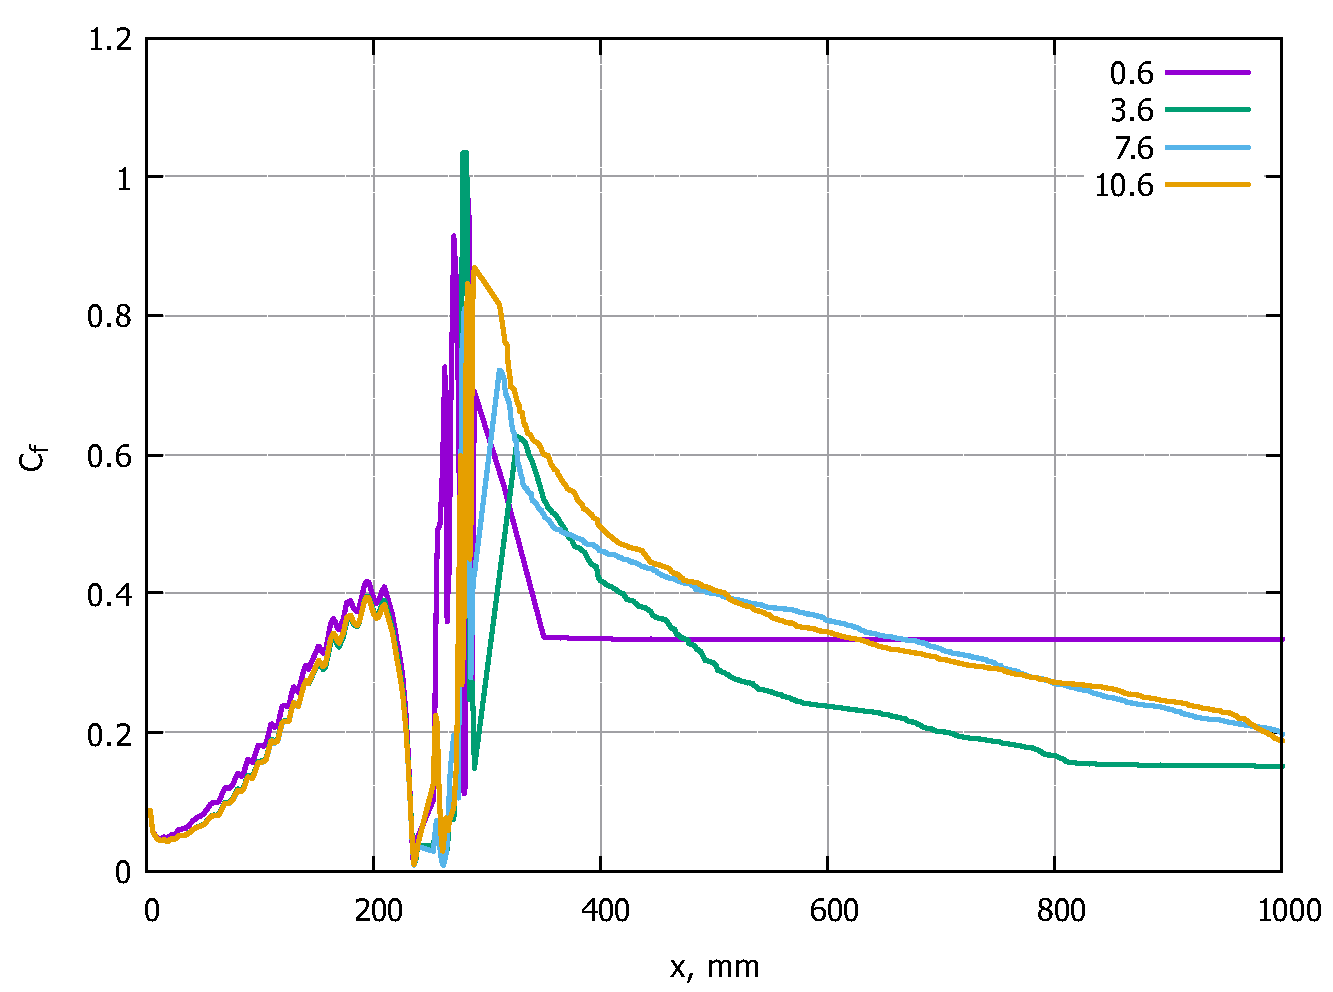
\includegraphics[width=0.9\linewidth]{../Assets/Cf-Tall}
	\caption{Изменение коэффициента трения по длине канала}
	\label{fig:cf-tall}
\end{figure}
\newpage
\begin{flushright}
	\MakeUppercase{\textbf{Приложение B}}
\end{flushright}
